\section{Тема 3. Теория массового обслуживания и её применимость в исследовании менеджмента}

Теория массового обслуживания представляет собой область прикладной математики, использующую методы теории случайных процессов и теории вероятностей для исследования различной природы сложных систем. Теория массового обслуживания непосредственно не связана с оптимизацией. Назначение ее состоит в том, чтобы на основе результатов наблюдений за «входом» в систему предсказать ее возможности и организовать наилучшее обслуживание для конкретной ситуации и понять, как последнее отразится на стоимости системы в целом. 

Для систем, относящихся к системам массового обслуживания, существует определенный класс задач, решение которых позволяет ответить на актуальные для сегодняшнего времени вопросы. С какой интенсивностью должно проходить обслуживание или должен выполняться процесс при заданной интенсивности и других параметрах входящего потока требований, чтобы минимизировать очередь или задержку в подготовке документа или другого вида информации? Какова вероятность появления задержки или очереди и ее величина? Сколько времени требование находится в очереди и каким образом минимизировать его задержку? Какова вероятность потери требования (клиента)? Какова должна быть оптимальная загрузка обслуживающих каналов? При каких параметрах системы достигаются минимальные потери прибыли? К этому перечню можно добавить еще целый ряд задач.

Система массового обслуживания (СМО) включает следующие структурообразующие объекты: источник требований; входной поток требований (поступление заявок); очередь; обслуживающую систему как совокупность каналов обслуживания заявок; выходной поток (обслуженные заявки или удовлетворенные требования). Рассмотрим их модели.

Источник требований. По месту нахождения источника, формирующего требования, СМО делятся на разомкнутые, когда источник находится вне системы, и замкнутые, когда источник находится внутри системы.

Входной поток требований. Подавляющее большинство теоретических разработок по исследованию систем массового обслуживания выполнено для условия, когда входной поток требований является пуассоновским (простейшим). Этот поток обладает рядом важных свойств. Он стационарен, ординарен и не имеет последствий.

Модель входного пуассоновского потока представляется функцией вида:
\[P_n(T) = \dfrac{(\lambda T)^ne^{\lambda T}}{n!},\]
где $ P_n(T)  $ --- вероятность поступления требований в течение заданного интервала времени $T$; \\
$\lambda$ --- интенсивность поступления требований в систему, т.е. математическое ожидание числа требований, поступивших за единицу времени:
\[\lambda =  \dfrac{1}{M(t)},\]
где $M(t)$ --- математическое ожидание случайной величины $t_i$, равной интервалу времени между $i$ и $i + 1$ поступлениями требований в систему; \\
$\lambda T$ --- математическое ожидание количества требований в период $T$; \\
$n$ --- количество поступлений требований в систему.

Следующее важное для исследования свойство, которым обладает пуассоновский поток, заключается в том, что процедура разделения и объединения дает снова пуассоновские потоки. Тогда, если входной поток формируется из $N$ независимых источников, каждый из которых порождает пуассоновский поток интенсивностью $\lambda_i (i=1,2,..., N),$ то его интенсивность будет определяться по формуле:
\[\lambda = \lambda_1 + \lambda_2 + ... + \lambda_N.\]

В случае разделения пуассоновского потока на $ N $ независимых потоков получим, что интенсивность потока $\lambda_i$ будет равна $r_i \lambda$, где $r_i$ --- доля $i$-го потока во входном потоке требований.

Очередь. Очереди, определяемые как множество требований, ожидающих обслуживания, представляются несколькими моделями: очередь с отказами, с ограниченным временем ожидания (заявка ждет определенное время), ограниченной длиной и, наконец, неограничен-ным временем ожидания. Порядок поступления заявок на обслуживание называется дисциплиной очереди. Требования могут приниматься по мере поступления, случайным порядком, с приоритетом, по принципу «последняя --- первой», по определенным каналам.

Процесс обслуживания. Основным параметром процесса обслуживания считается время обслуживания требования каналом $j$ --- $t_j(j =1,2,...,m)$. Величина $\uptau_j$ в каждом конкретном случае определяется рядом факторов: интенсивностью поступления заявок, квалификацией исполнителя, технологией работ, окружающей средой и т.д. Законы распределения случайной величины $\uptau_j$ могут быть самыми различными, но наибольшее распространение в практических приложениях получил экспоненциальный закон распределения. Функция распределения случайной величины $\uptau_j$ имеет вид:
\[F(t)=1-e^m,\]
где $m$ --- положительный параметр, определяющий интенсивность обслуживания требований;
\[m=\dfrac{1}{E(t)},\]
где $E(t)$ --- математическое ожидание случайной величины обслуживания требования $\uptau_j$.

Важнейшее свойство экспоненциального распределения заключается в следующем. При наличии нескольких однотипных каналов обслуживания и равной вероятности их выбора при поступлении заявки распределение времени обслуживания всеми $m$ каналами будет показательной функцией вида:
\[F(\uptau) = 1-e^{(\mu_1 +\mu_2 + ... + \mu_m)_{\uptau}}.\]

Если СМО состоит из неоднородных каналов, то $\mu = \sum\limits_{j=1}^m\mu_j$, если же все каналы однородные, то $\mu = m \mu_j$.

Выходной поток обслуженных требований. Выходной поток — это поток результатов деятельности, представленных выполненными требованиями в виде той или иной продукции или услуги. К основным параметрам выходного потока относятся интенсивность выхода из системы обслуженных требований и характер распределения времени между моментами выпуска продукции. В общем случае эти параметры определяются моделью входного потока, дисциплиной очереди и моделью обслуживания. Для СМО с параллельными каналами и однофазным обслуживанием существует теорема о том, что при пуассоновском входном потоке с параметром $\lambda$ и одинаковым для каждого канала распределением времени обслуживания с параметром $\mu$ в стационарном состоянии выходной поток имеет пуассоновское распределение с параметром $g$. В многофазных системах выходной поток одного канала служит входным потоком для другого канала. Параметр $g$ в простейшем случае определяется по формуле:
\[g=\dfrac{1}{W_s},\]
где $W_s$ --- среднее время пребывания требования в системе.

Особенность моделей СМО связана с достаточно строгим математическим описанием функционирования систем, что достигается благодаря их унификации по ряду признаков. Так, в зависимости от модели ожидания требованием начала обслуживания различают следующие СМО:
\begin{itemize}
	\item системы с потерями или отказами;
	\item системы с ожиданием;
	\item системы с ограниченным временем ожидания (ВО);
\item системы с ограниченной длиной очереди (ДО).
\end{itemize}

По числу каналов обслуживания системы делятся на одноканальные ($m = 1$) и многоканальные ($m > 1$). Структура СМО и характеристика ее объектов приведены на рисунке \ref{fig:}.

\begin{figure}[!h]
	\centering
	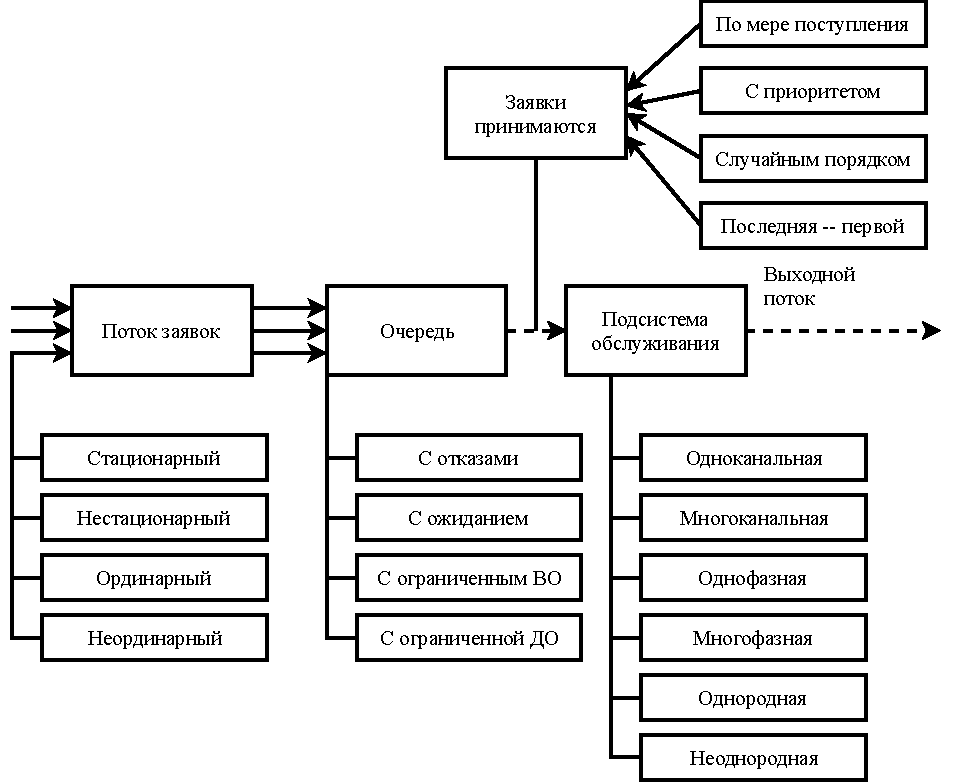
\includegraphics{smo}
	\caption{Структура и характеристика объектов СМО}
	\label{fig:}
\end{figure}


Одной из форм классификации СМО служит кодовая классификация Д. Кендалла. В соответствии с этой классификацией характеристику СМО записывают в виде трех, четырех или пяти символов. Например, $ а/Ь/с $, где $ a $ --- тип распределения входного потока требований, $ b $ --- тип распределения времени обслуживания, $ с $ --- число каналов обслуживания. Для пуассоновского и экспоненциального распределений принимают символ $M$, для любого произвольного распределения --- символ $ M $. Например, запись $ М/М/2  $означает, что входной поток требований пуассоновский, время обслуживания распределено по экспоненциальному закону, в системе имеются два канала. Четвертый символ $ (d) $ указывает допустимую длину очереди, пятый $ (e) $ --- порядок отбора требований.

Модели СМО могут быть детерминированными или вероятностными. В первом случае параметры и переменные модели --- это постоянные величины, во втором --- случайные.

Исследование СМО заключается в нахождении показателей, характеризующих качество и условия работы обслуживающей системы и показателей, отражающих экономические последствия принятых решений согласно первым показателям. К показателям первой группы относятся следующие.

1. При установленных или проектных параметрах входящего потока:\\

а) вероятность поступления $n$ требований в систему за период $t(P_n(T))$;\\

б) вероятность наличия $n$ требований в системе $(P_n).$\\


Рассмотрим приемы вычисления показателей первой группы на примере наиболее распространенной модели СМО (М/М/т > 2) с ожиданием, содержащей т параллельных обслуживающих каналов. Здесь поступающие требования не теряются и оставляют систему лишь после обслуживания. Каналы выполняют однородные операции, и время обслуживания каждым каналом * распределено по экспоненциальному закону с параметром т (10.5), а входящий поток — пуассоновский с параметром X (10.1); дисциплина очереди не регламентирована, и отсутствует ограничение на число поступающих требований. Модель СМО представляется в виде системы уравнений для стационарного состояния.

Пример. Требуется провести оценку эффективности централизации нескольких отделов или служб с однородными функциями. В качестве объекта рассматриваются две службы такси, которые приобрела компания «Автосервис». Заявки клиентов между службами распределяются поровну. Спрос на такси к диспетчеру поступает с частотой 10 вызовов в час. Среднее время обслуживания одного клиента составляет 11,5 мин. Вызовы такси распределены во времени по пуассоновскому закону, а продолжительность обслуживания одного клиента — по экспоненциальному закону. Каждая служба такси оснащена двумя автомобилями.

Возникает вопрос об экономической целесообразности централи-зации управления таксопарком. Для этого необходимо сравнить два варианта:
\begin{enumerate}
	\item вариант с независимым обслуживанием системами типа (М/М/2) при51= 10 вызовов/ч,т = 11,5мин. ит = 2;
	\item вариант с одной очередью типа (М/М/4) при X = 10 • 2 = 20 вызовов /ч, т — 11,5 мин. и /и = 4.
\end{enumerate}

Приведенные оценки показывают, что централизация служб позволяет сократить среднее время ожидания клиентом вызванного по телефону такси примерно вдвое. Это не гарантия, что клиент откажется от заказа, но существенное сокращение времени ожидания. В дальнейшем, кроме создания единой службы такси, необходимо рассматривать вопросы увеличения парка такси. При решении задач с размерностью т > 5 методами теории массового обслуживания потребуется автоматизированное вычисление.

Подводя итоги, отметим, что теория массового обслуживания предоставляет исследователю множество разнообразных моделей и методов решения задач по повышению эффективности обслуживания по-
требителей, клиентов.